\chapter{Preliminary Data and Future Outlook}\label{s:Prel}

Figure~\ref{Fig:pathfinderresults} shows the results from the two interferometric array pathfinder discussed in \S\ref{s:pathfinder}. These results were an encouraging factor to proceed with the development of the autonomous stations. Figure~\ref{Fig:pathfinderresults} shows the auto- and cross- spectra where the waterfall plot was taken from one polarization over three days (June 18–21, 2018). The Galaxy rising/setting is visible in the structure. There are also ripples in frequency because of uncalibrated data, and the ripples arise from reflections in the cables. There is a qualitative difference between daytime and nighttime data, and this shows that the contamination from shortwave radio drops off significantly at night, when the ionosphere becomes quieter. It is distinctly visible from the figure that fringes show recurrent structure below $\sim$ \SI{10}{\mega\hertz} without data processing or data cuts. The auto spectra signal drop-off below $\lesssim$\SI{ 30}{\mega\hertz} results from the combined response of the antenna and the front-end electronics as shown in Figure~\ref{Fig:s11lwa}.

\begin{figure}
	\centering
	\includegraphics[width=0.9\linewidth]{"Figures/pathfinder results"}
	\caption{Spectra from a two-element ALBATROS pathfinder co-aligned polarization pair, shown as a frequency and time function. In the top and bottom rows, the auto- and cross-spectra are shown, respectively. The spectrum magnitudes are in uncalibrated ADC units on a logarithmic scale, and the amplitude of the cross-spectrum is around two orders of magnitude fainter than the auto spectra. The phase of the cross-spectrum can be seen in radians. The Galaxy's repeatable structure is evident in all plots over the 3-day time scale.}
	\label{Fig:pathfinderresults}
\end{figure}

\begin{figure}
	\centering
	\includegraphics[width=0.9\linewidth]{"Figures/s11 lwa"}
	\caption{Top: LWA antenna simulated S11, demonstrating the steep loss of signal below \SI{\sim 30}{\mega \hertz}. Bottom panel: for one of the polarization in the two-element ALBATROS pathfinder, the median uncalibrated auto spectrum compared to the crude sky signal estimate provided by the product (1-S11) with the product spectrum of nominal synchrotrons. Qualitatively, this simple model shows that the reduction in the antenna response is primarily responsible for auto spectrum power below \SI{\sim 30}{\mega \hertz}.}
	\label{Fig:s11lwa}
\end{figure}

An approximation of the instrumental consistency in gain can be obtained by comparing the total power between various days illustrated in Figure~\ref{Fig:pathfinderresults}. Within the frequencies of 30 and 40 MHz, it has been discovered that the RMS gain variations are below \SI{1}{\percent} and approximately \SI{0.04}{\percent} of the power at the standard noise on time scales of 3 seconds. The minimal noise indicates that relative calibration will yield sub-percent accuracy using auto spectra reported by each autonomous station. In the future, outright calibration will be extracted from the contrast of auto spectra with the co-located and thoroughly calibrated \prizm\ or Global Sky Model. Figure~\ref{Fig:pol1} shows the cross-spectra phases binned in nearby sidereal time as a subjective representation of the sky signal repeatability on tiny scales.

In this plot, about 372 hours of data are averaged, and no RFI extraction has been carried out. The high signal-to-noise fringe pattern, which is noticeable even marginally beneath $\sim$\SI{10}{\mega\hertz}, shows the verification of an idea for extending the ALBATROS array.

\begin{figure}
	\centering
	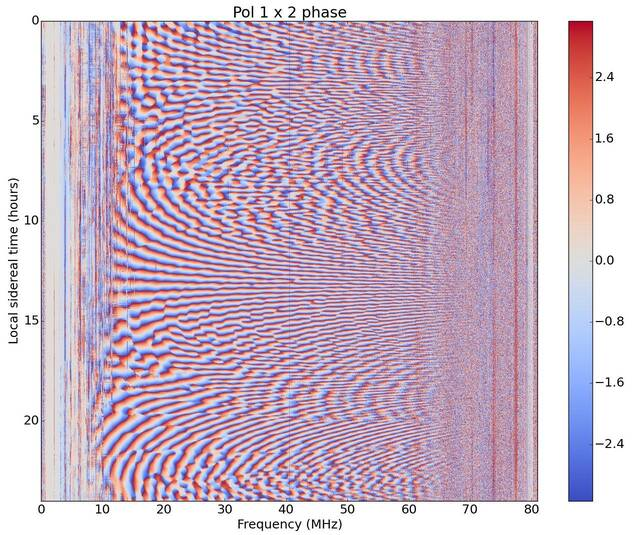
\includegraphics[width=0.7\linewidth]{Figures/pol1}
	\caption{Phases from the cross-correlation in the two-element ALBATROS pathfinder between two co-aligned polarizations. There are approximately 372 hours of data displayed here, binned in local sidereal time, and radians are the color stretch.}
	\label{Fig:pol1}
\end{figure}

Due to COVID-19 restriction and limited accessibility to the island, the data could not be retrieved from the single autonomous station pathfinder on Marion discussed in \S\ref{s:autonomous}; however, verification of the solar power system has effectively met the antenna station's power requirements. Because of the unavailability of data from Marion, baseband writing has been demonstrated by setting up a single-element pathfinder station at the McGill Arctic Research Station (MARS; \ang{79;26;}N, \ang{90;46;}W) Axel Heiberg Island, Nunavut, in July 2019. The RF signal chain shown in Figure~\ref{Fig:albatros1_schem} is similar to the MARS installation; although a solar power system was not used, instead manually charged batteries were used to supply power. The MARS RFI atmosphere is much noisier than that of Marion Island. The ionospheric plasma cutoff frequency is higher than the average cutoff displayed in the Marion data because the data was taken during the peak of the Arctic summer. The MARS installation is appropriate for demonstrating baseband data writing, regardless of the distinct layout and RFI environment. 

Short chunks of baseband data that have been collected at different times over two adjoining frequency windows are displayed, \SIrange{5.3}{12.6}{\mega \hertz} and \SIrange{12.6}{20}{\mega \hertz}. In order to maintain auto spectrum data, the baseband data was registered with 4-bit quantization, which is not obtainable with 1-bit quantization. The one polarization auto spectra from the ALBATROS single-element pathfinder station that was set-up at MARS is shown in Figure~\ref{Fig:mars}, looking at the aggregated spectra that are directly registered by the SNAP board versus the spectra determined from baseband data. Altogether, the waterfall plots have the same 61-kHz frequency resolution, as defined by the spectrum resolution measured by the SNAP board. A logarithmic scale is shown in the waterfall plots to demonstrate the qualitative agreement for bright and faint spectral characteristics between the directly accumulated and baseband spectra. In order to demonstrate variations in the striking RFI characteristics that immerse the baseband data, the bottommost panels display the time-averaged spectra on a linear scale. Except where major immersion is present, the portion of baseband data with values at the 4-bit extrema is over-plotted with spectra. There is an understanding between the directly accumulated and baseband spectra. Figure~\ref{Fig:crossmars} shows waterfall phase plots calculated from the cross-correlation between two orthogonal polarizations of the ALBATROS pathfinder at MARS, looking at the directly accumulated and baseband data. Qualitatively, both sets of reported data concur, down to minor variations induced by the 4-bit quantization.

\begin{figure}
	\centering
	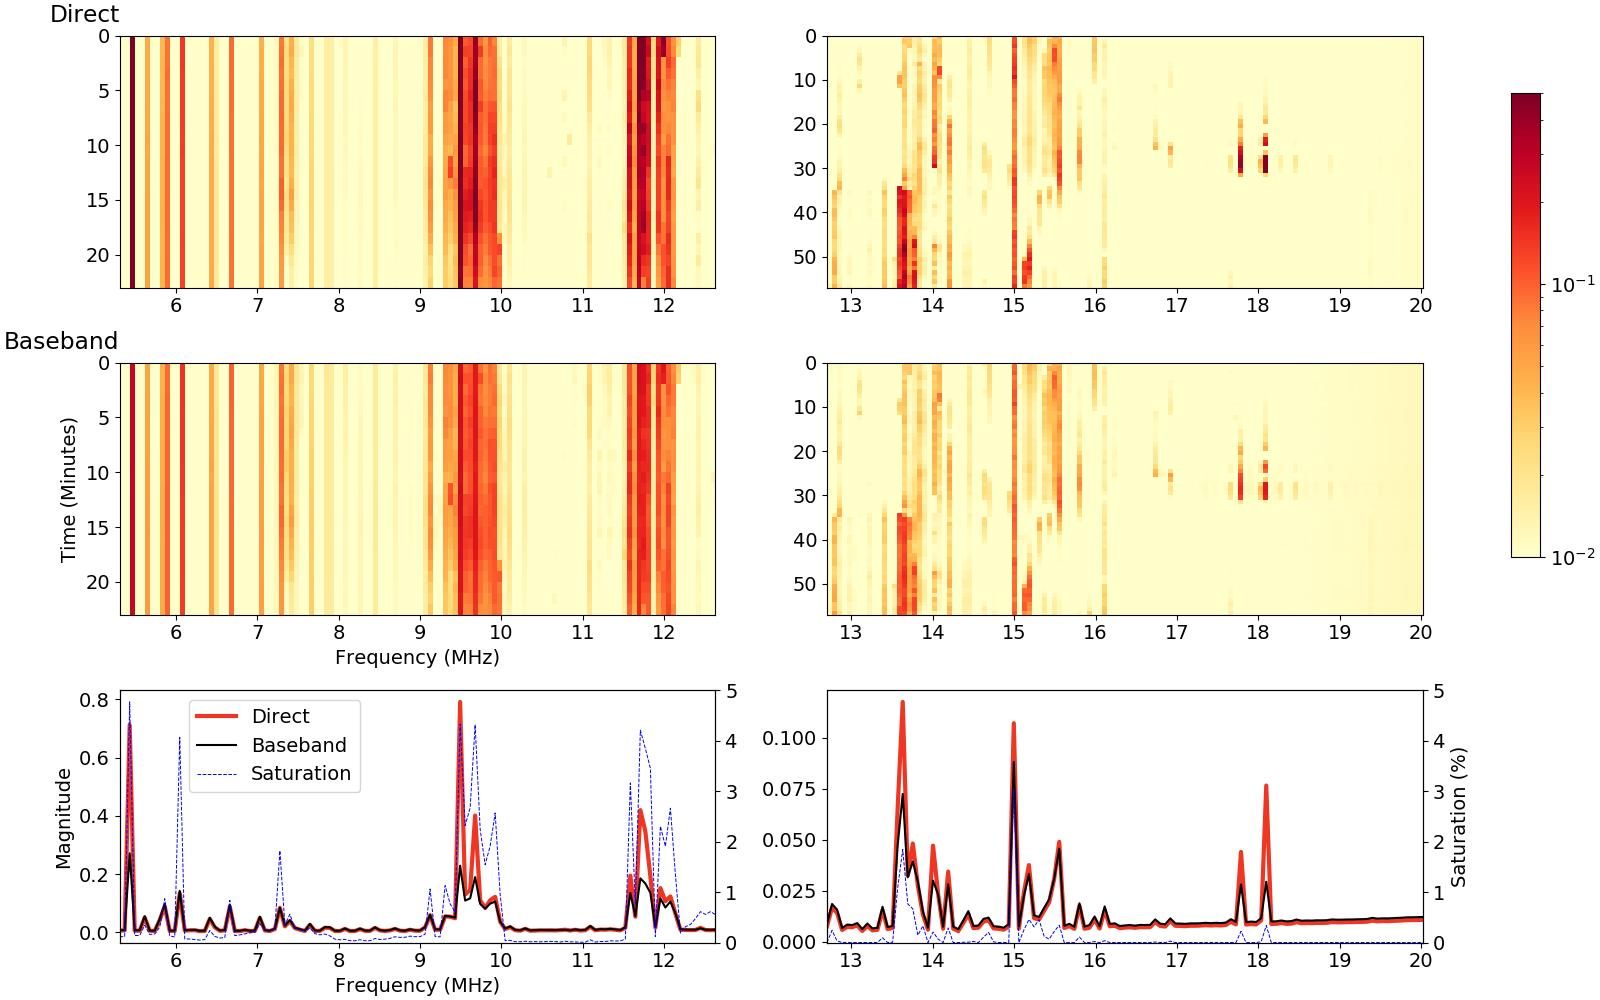
\includegraphics[width=\linewidth]{Figures/mars}
	\caption{Autospectra from the ALBATROS pathfinder at MARS for one polarization. The top row shows spectra directly accumulated by the SNAP board, and the middle row displays spectra with 4-bit quantization computed from baseband data. The two frequency windows are registered at two different periods, 5.3-12.6 MHz and 12.6-20.0 MHz, and both plots are displayed at a 61-kHz resolution.}
	\label{Fig:mars}
\end{figure}

\begin{figure}
	\centering
	\includegraphics[width=\linewidth]{"Figures/cross mars"}
	\caption{Cross-correlation phases between two orthogonal polarizations from the  ALBATROS pathfinder at MARS. The top row shows cross-spectrum phases that are directly accumulated by the SNAP board, and the bottom row shows phases with 4-bit quantization computed from baseband results. The two frequency windows, \SIrange{5.3}{12.6}{\mega \hertz} and \SIrange{12.6}{20}{\mega \hertz} are registered at two different times, and all 61-kHz resolution waterfall plots are shown.}
	\label{Fig:crossmars}
\end{figure}


\section{Conclusion and Future Outlook}

The design of \albatros\, a new interferometer that will image the radio sky at \SI{\sim 30}{\mega \hertz} using an array of autonomous antenna stations installed on Marion Island, has been presented. A clear demonstration of the repeatable sky signal visible from Marion down to $\lesssim$10~MHz without data processing or cutting, with a two-element, directly correlated pathfinder. The first autonomous prototype for \albatros\ powered solar panels have been constructed, and the electronics and database recording software have been successfully tested.

There are plans to improve the design of the future \albatros\ stations to be deployed in the coastal huts of Marion, with the evidence of the concept shown in the pathfinder instruments presented here. Currently, the LWA and FEE antennas are not designed for the lowest \albatros\ frequency observation, and potential antenna and FEE design modifications are being explored to enhance the low-frequency response of the calibration circuitry construction. Since future \albatros\ stations would be located farther away from the base and will be more challenging to access regularly, to store baseband data over extended periods, each station will require larger total disk space. A specially made low-power hard disk drive bank is being developed with $>$ 100~TB total capacity, and a USB multiplexer will be used to select and power only one hard drive at a time. The autonomous pathfinder of the station presented uses solar panels to charge the batteries and, as a future alternative for potential stations, the use of small wind turbines is explored. To compute time-domain data from the recorded channelized baseband, analysis tools are being built by inverting the polyphase filter bank while minimizing quantization and saturation artifacts.

A proposal for building a second \albatros\ array at MARS shown in Figure~\ref{Fig:MARS} in the high Arctic is being studied in addition to Marion Island. In July 2019, a single pathfinder antenna was mounted as defined in \S\ref{s:Prel} and observed for about three weeks to evaluate the RFI environment and ionospheric conditions. When fully operational, Marion and MARS \albatros\ will have new views across both hemispheres of the low-frequency sky.

\begin{figure}
	\centering
	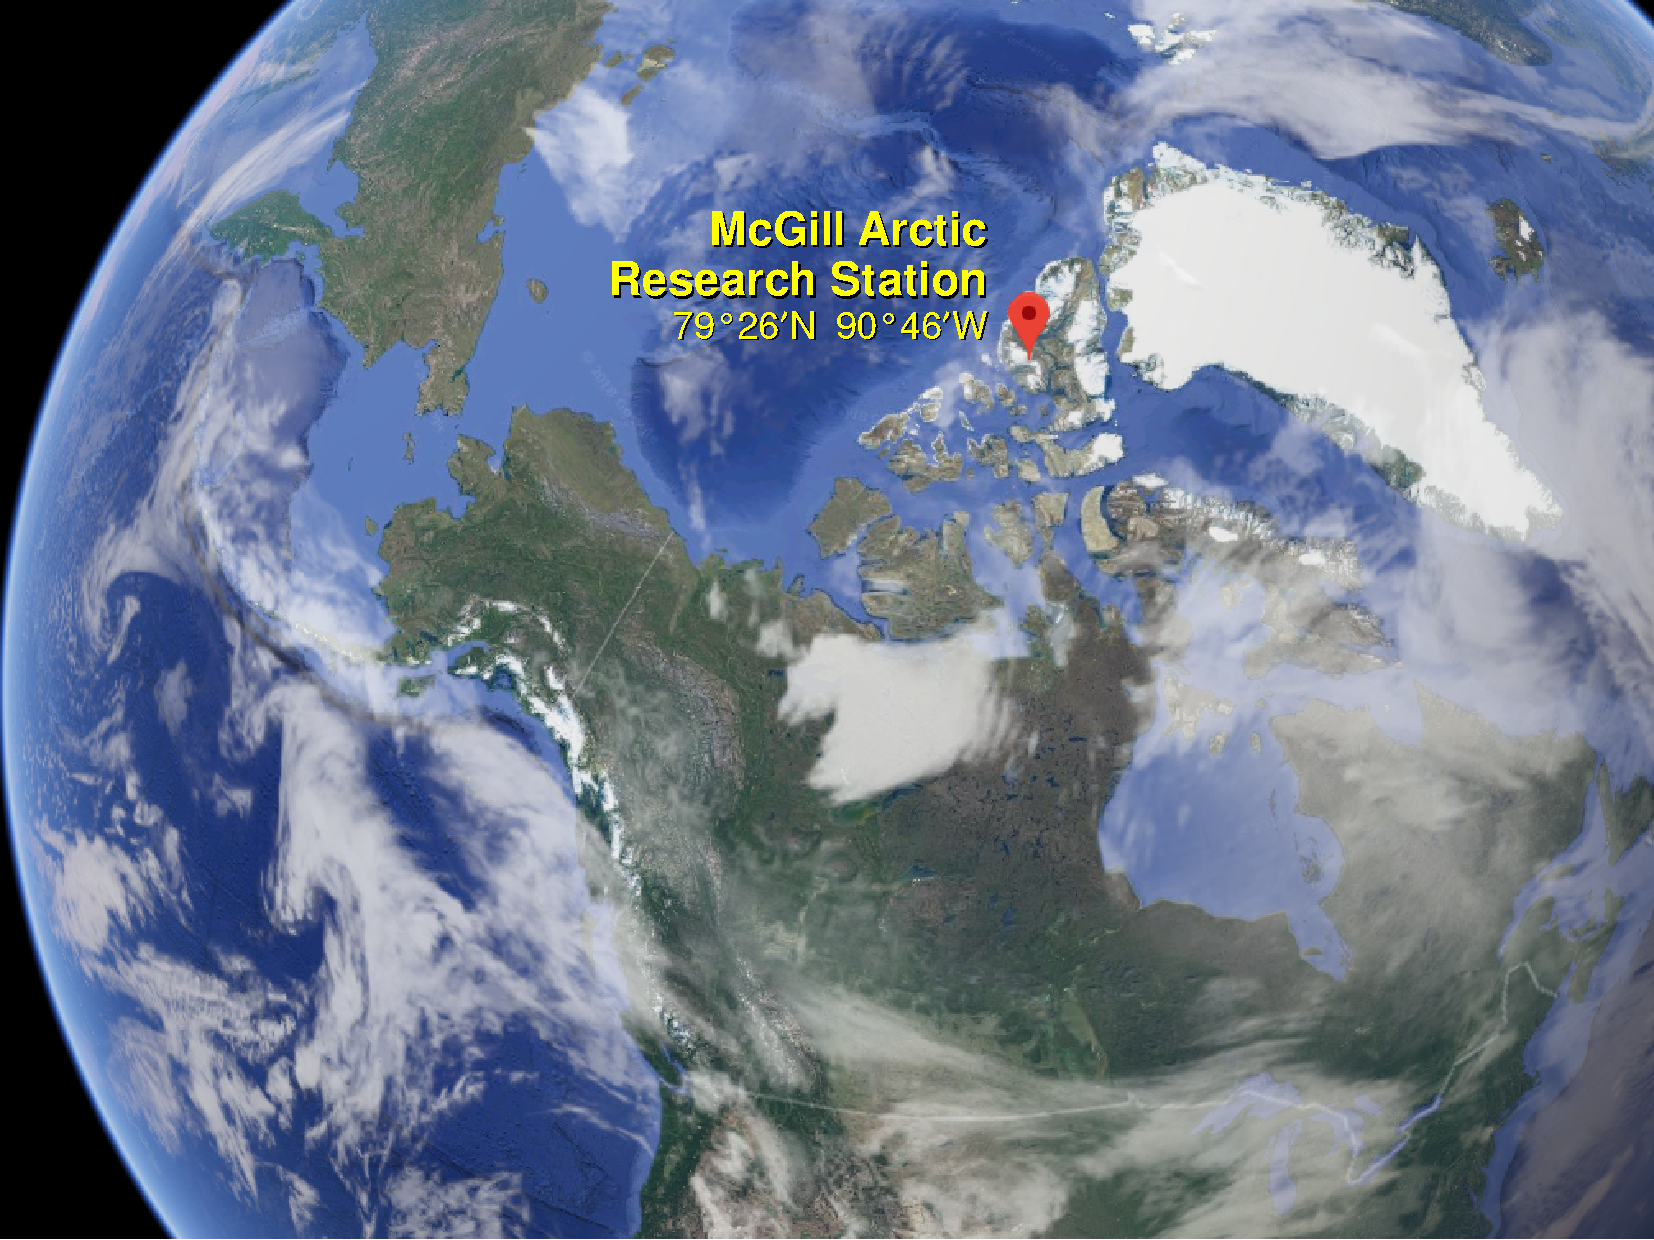
\includegraphics[width=\linewidth]{Figures/MARS}
	\caption{The world map showing the location of MARS, where the \albatros\ will be viewing the Northern hemisphere sky.}
	\label{Fig:MARS}
\end{figure}

The \prizm\ experiment which was the first radio astronomy project in Marion Island was discussed and the revision of the subsystems was clearly presented. The new FSE was designed and further modifications are still going to be employed. The SSE enclosure was successfully designed, fabricated and the enclosure parts were fitted together. The design of the new switch control circuit was successful and it fitted the stacked layout on top of the RPi. All the \prizm\ modifications are still going to be employed on the next Marion voyage, hopefully in April 2021. 